\documentclass[tikz,14pt]{standalone}

\usetikzlibrary{arrows, automata}

\begin{document}

    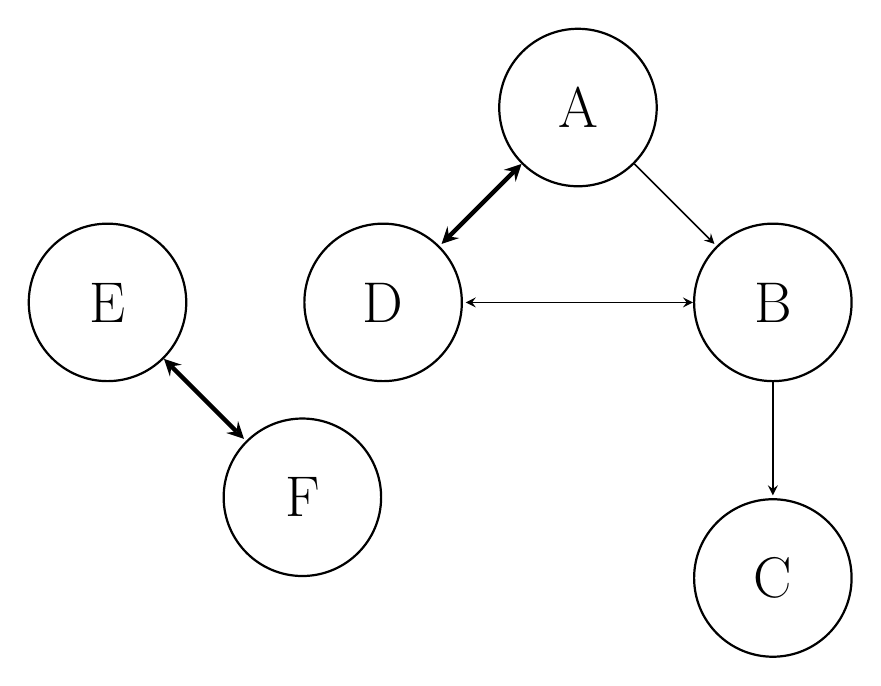
\begin{tikzpicture}[
            > = stealth, % arrow head style
            shorten > = 1pt, % don't touch arrow head to node
            auto,
            node distance = 3.5cm, % distance between nodes
            semithick % line style
        ]

        \tikzstyle{every state}=[
            draw = black,
            thick,
            fill = white,
            minimum size = 2cm,
            font = \huge
        ]

        \node[state] (A) {A};
        \node[state] (B) [below right of=A] {B};
        \node[state] (C) [below of=B] {C};
        \node[state] (D) [below left of=A] {D};
        
        \node[state] (E) [left of=D] {E};
        \node[state] (F) [below right of=E] {F};

        \path[->] (A) edge node {} (B);
        \path[<->, ultra thick] (A) edge node {} (D);
        \path[<->] (B) edge node {} (D);
        \path[->] (B) edge node {} (C);
        \path[<->, ultra thick] (E) edge node {} (F);
        
    \end{tikzpicture}

\end{document}